%%%%%%%%%%%%%%%%%%%%%%%%%%%%%%%%%%%%%%%%%
% Diaz Essay
% LaTeX Template
% Version 2.0 (13/1/19)
%
% This template originates from:
% http://www.LaTeXTemplates.com
%
% Authors:
% Vel (vel@LaTeXTemplates.com)
% Nicolas Diaz (nsdiaz@uc.cl)
%
% License:
% CC BY-NC-SA 3.0 (http://creativecommons.org/licenses/by-nc-sa/3.0/)
%
%%%%%%%%%%%%%%%%%%%%%%%%%%%%%%%%%%%%%%%%%

%----------------------------------------------------------------------------------------
%	PACKAGES AND OTHER DOCUMENT CONFIGURATIONS
%----------------------------------------------------------------------------------------



\documentclass[11pt]{diazessay} % Font size (can be 10pt, 11pt or 12pt)



%----------------------------------------------------------------------------------------
%	TITLE SECTION
%----------------------------------------------------------------------------------------

\title{\textbf{El juego de la vida} \\ {programación}} % Title and subtitle

\author{\textbf{Juan Manuel Velásquez Cadavid} 
\\
\textit{Modelado Matemático I}
\\ 
\textit{Maestría en Matemática Aplicada}
\\
\textit{Escuela de Física}
\\
\textit{Facultad de Ciencias}
\\ 
\textit{Universidad Industrial de Santander}} % Author and institution
\date{\today} % Date, use \date{} for no date

%----------------------------------------------------------------------------------------

\begin{document}

\begin{figure}[h!]

\includegraphics[scale=0.35]{Figures/uis}
\end{figure}

\maketitle % Print the title section

En el presente documento se explica brevemente el algoritmo del código contruido para el ``juego de la vida'', y se muestran algunos resultados interesantes. 

\section{El algoritmo}

El código está escrito de tal forma que el usuario ingresa la dimensión del tablero (filas y columnas), el número de las generaciones que desee evolucionar y la semilla de números aleatorios. Con esto, se genera una matriz binaria (rellena de unos y ceros) pseudoaleatoria de acuerdo a la semilla ingresada, de tal forma que se obtenga una matriz distinta al cambiar la semilla (en esta configuración no se toman en cuenta los bordes del tablero, es decir, siempre estarán en estado 0). Esta matriz inicial (generación 0) pasa a una función que determina el estado de las celdas al desplazarla en las ocho direcciones posibles. Una vez determinado el estado de todas las celdas, una función evolución itera el número de generaciones ingresado por el usuario y actualiza la matriz con los valores acordes a las condiciones del juego:
%
\begin{enumerate}
\item[1.] Una celda ``viva'' (etiquetada con el número 1) permanece viva si tiene dos o tres compañeras vivas. De lo contrario muere por soledad o sobrepoblación.
%
\item[2.] Una celda ``muerta'' (etiquetada con el número 0) nace si tiene exactamente tres vecinas vivas.
\end{enumerate}
%
En cada paso de generación se salvan los datos del número de celdas vivas, el número de celdas que murieron y el número de celdas que nacieron. Así mismo, las imágenes de cada evolución se guardan en cada ciclo, y al acabar las iteraciones también lo hace una gráfica de los parámetros anteriormente mencionados en función de la generación. Para probar el algoritmo se empleó una prueba con la configuración inicial mostrada en la figura \ref{fig:ini}
%
\begin{figure}[h!]
\centering
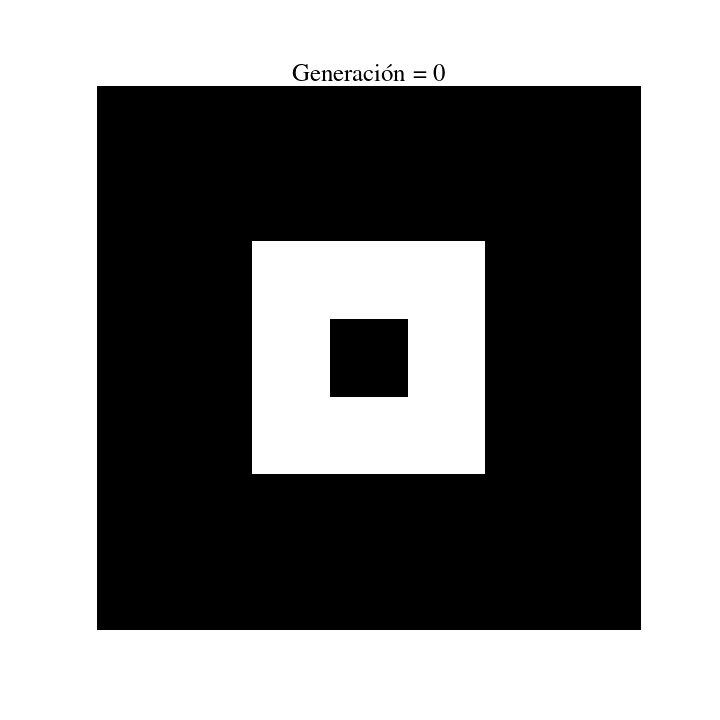
\includegraphics[scale=0.25]{prueba1}
\caption{configuración de prueba.} \label{fig:ini}
\end{figure}
\\
%
\begin{figure}[h!]
\centering
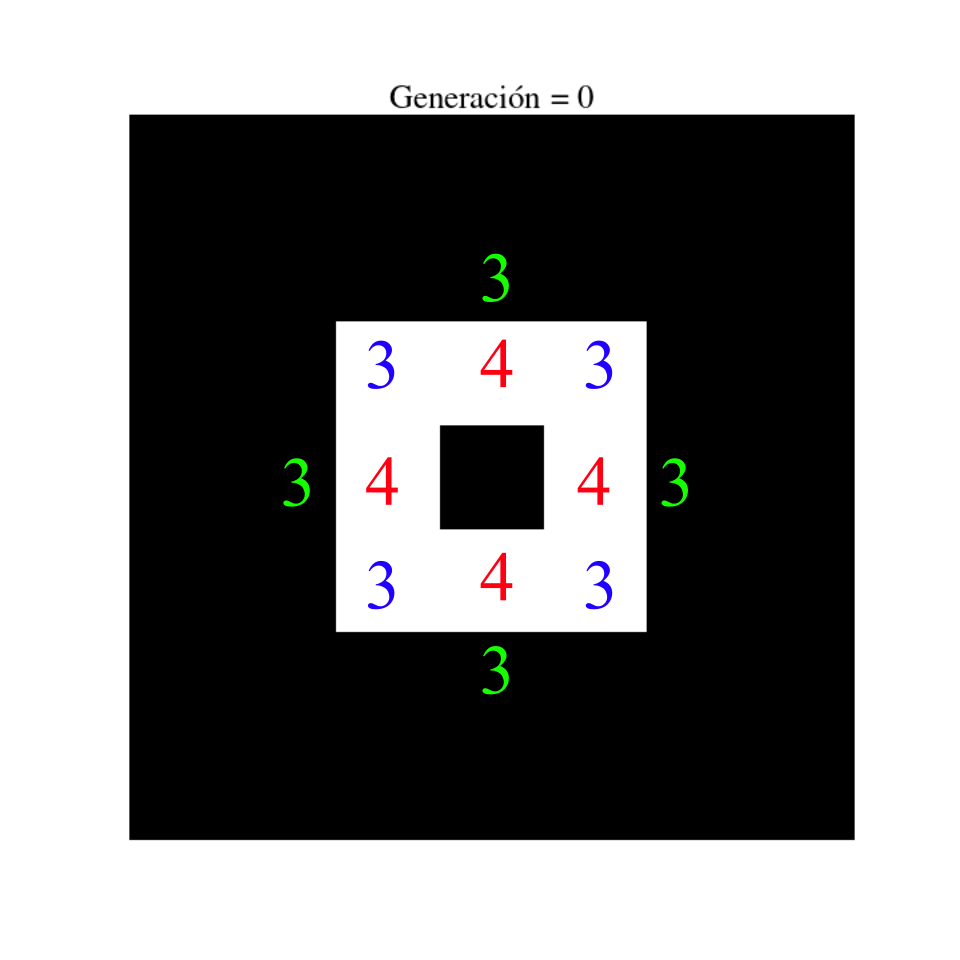
\includegraphics[scale=0.25]{prueba12}
\caption{estados de la configuración de prueba.}
\label{fig:est}
\end{figure}
\\
En la figura \ref{fig:est} pueden observarse los vecinos de las celdas de la matriz que determinarán su estado en la siguiente generación. El color verde indica el número de celdas ``muertas'' con tres vivas vecinas, por lo que nacerán en la generación siguiente; en azul están las celdas vivas que permanecerán en dicho estado en el cambio de generación, y en rojo aquellas que morirán. De esta forma se obtiene el patrón de la figura \ref{fig:gen1}. Con esto, el patrón generado por esta configuración se vuelve cíclico a partir de la tercera generación, como se muestra en la figura \ref{fig:gen_c}
%
\begin{figure}[h!]
\centering
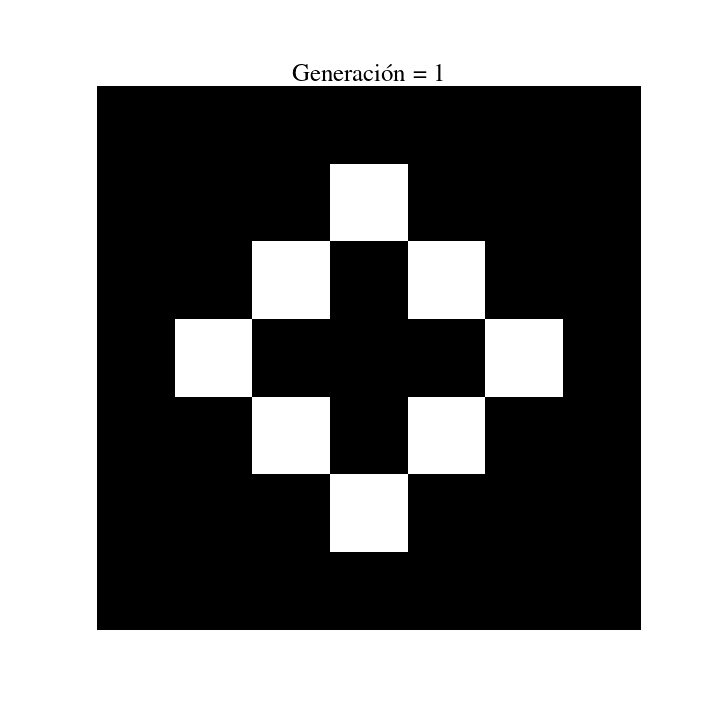
\includegraphics[scale=0.25]{prueba2}
\caption{configuración de prueba en la primera generación.} \label{fig:gen1}
\end{figure}
%
\begin{figure}[h!]
\centering
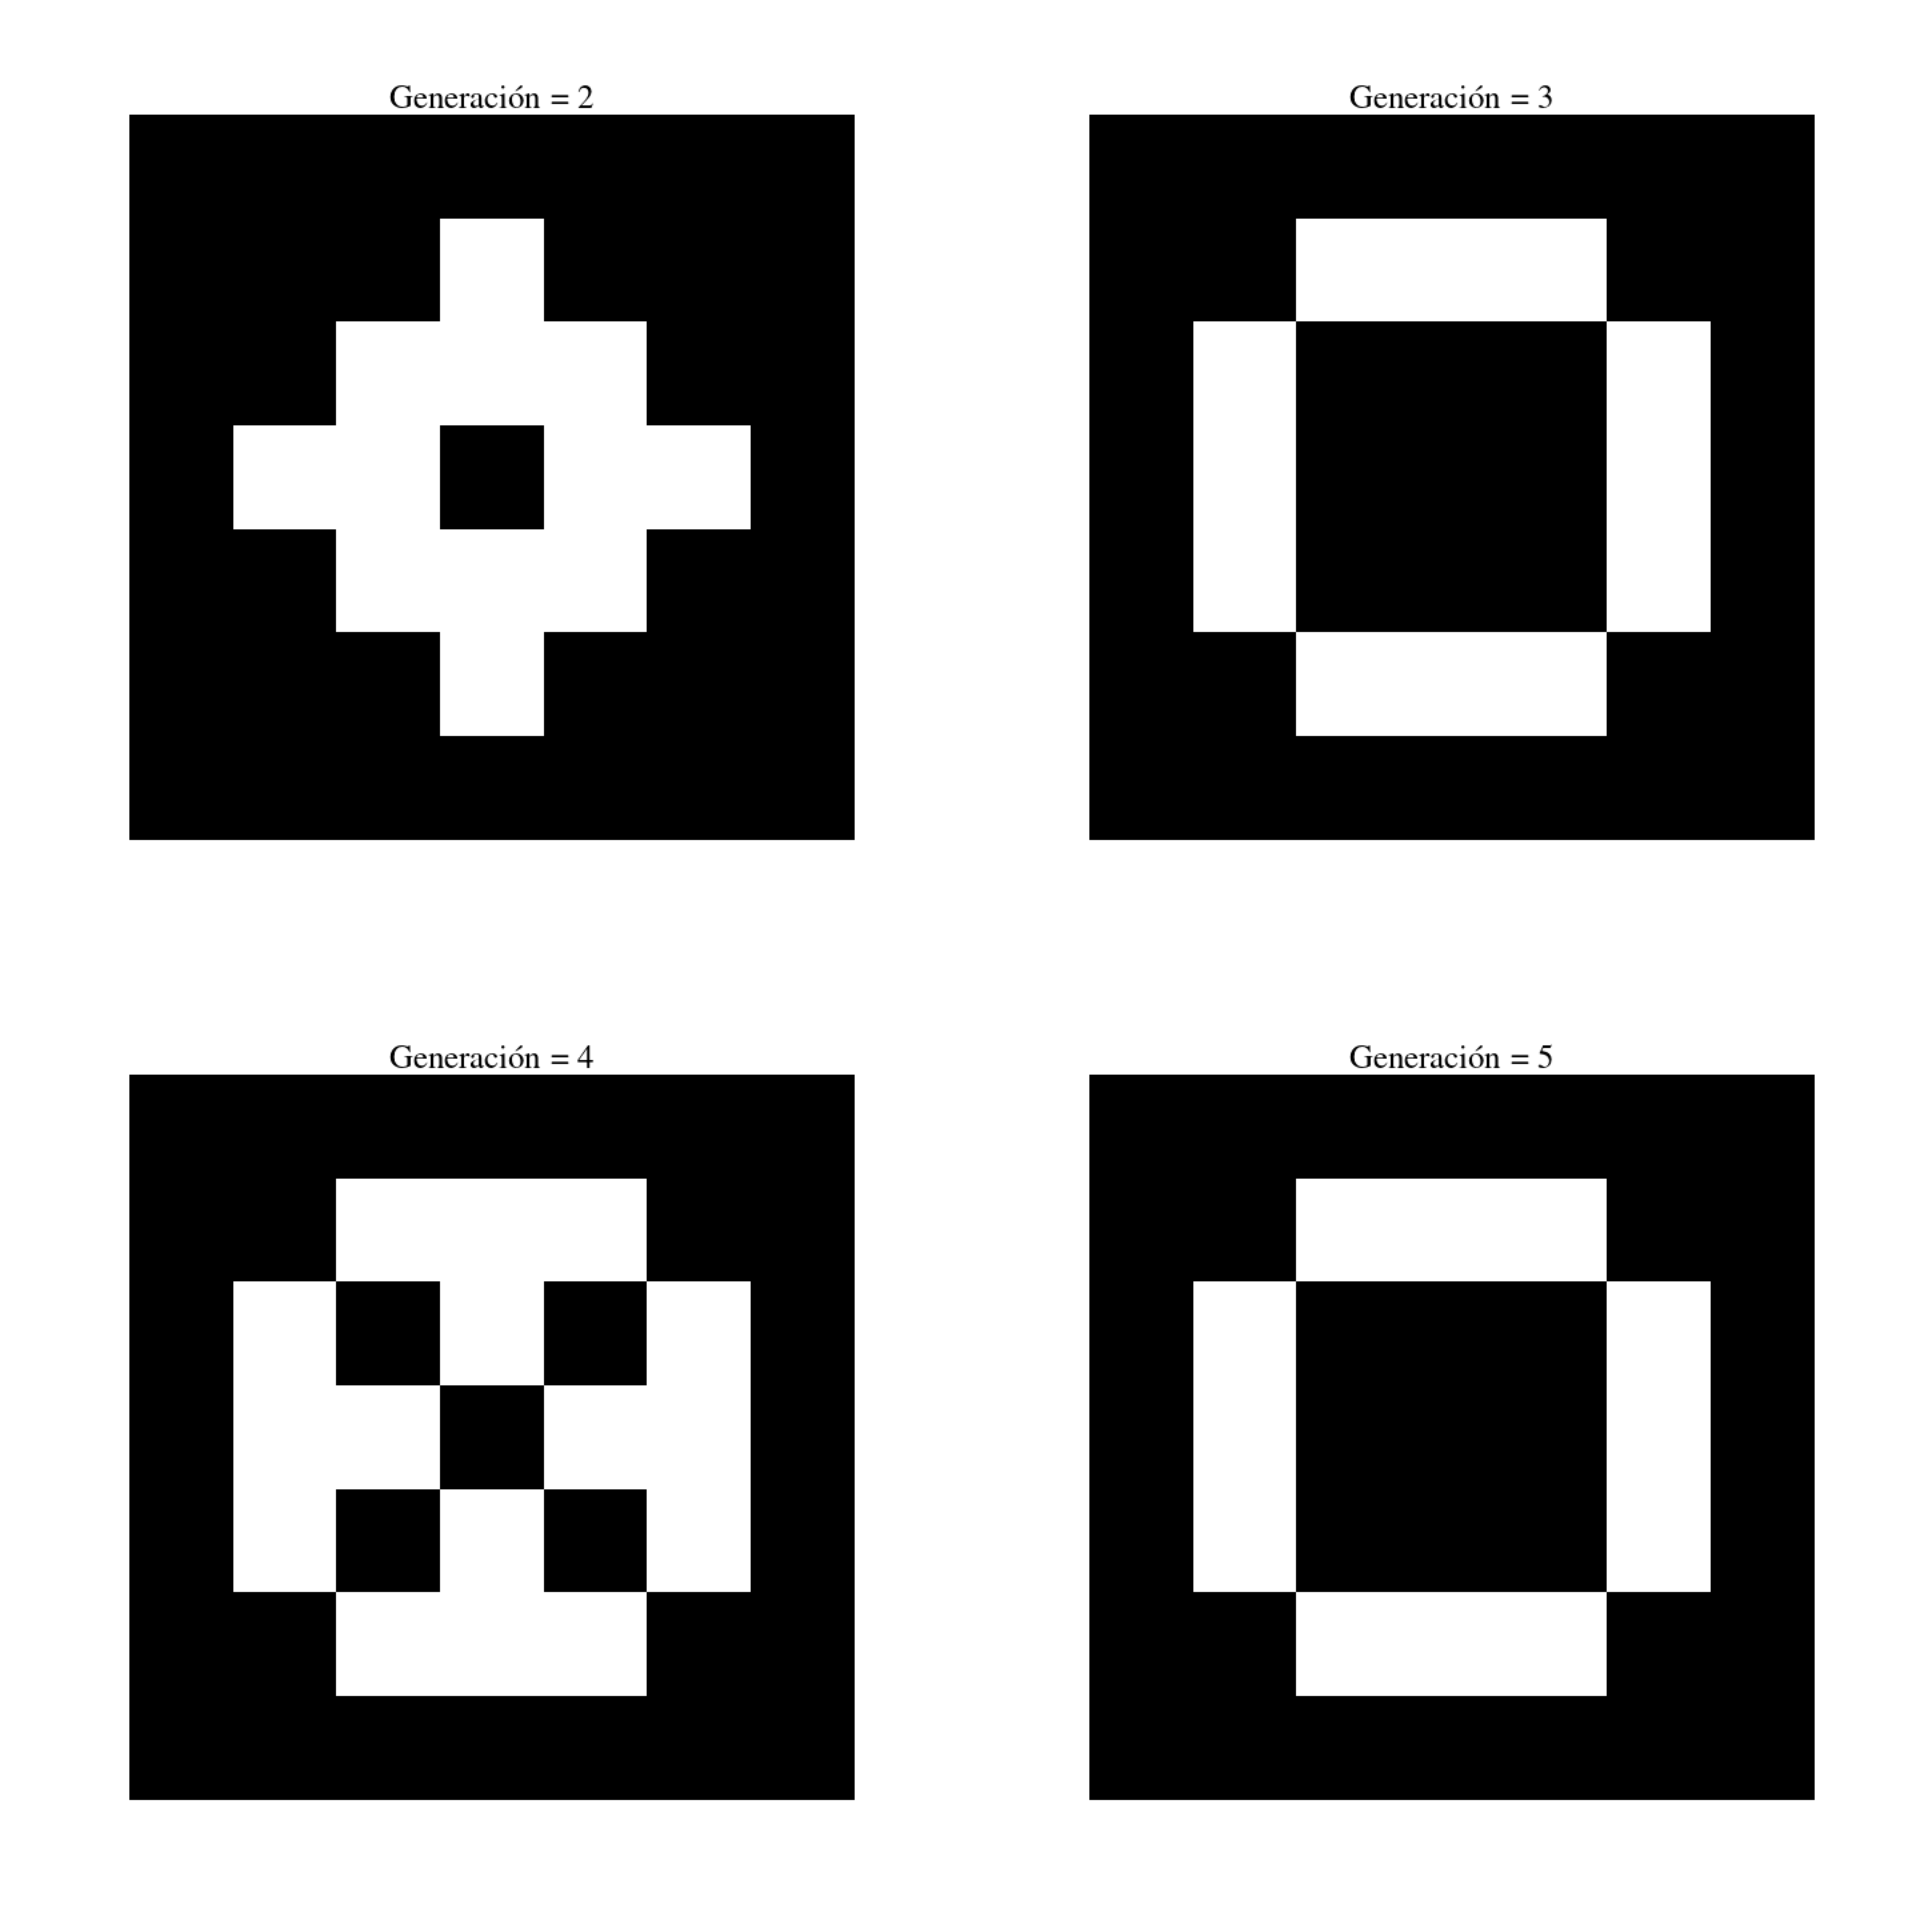
\includegraphics[scale=0.25]{prueba_p}
\caption{configuración de prueba en estado cíclico.} \label{fig:gen_c}
\end{figure}
%
\newpage
%
Con el algoritmo funcionando, se empleó una configuración de dimensión $dim = 100$, generación $gen = 100$ y semilla $seed = 1$, de lo cual se obiente la configuración inicial de la figura \ref{fig:gen_0}, cuya población viva es de 4786 celdas. Al concluir las cien iteraciones, el resultado final es el mostrado en la figura \ref{fig:fin}.
%
\begin{figure}[h!]
\centering
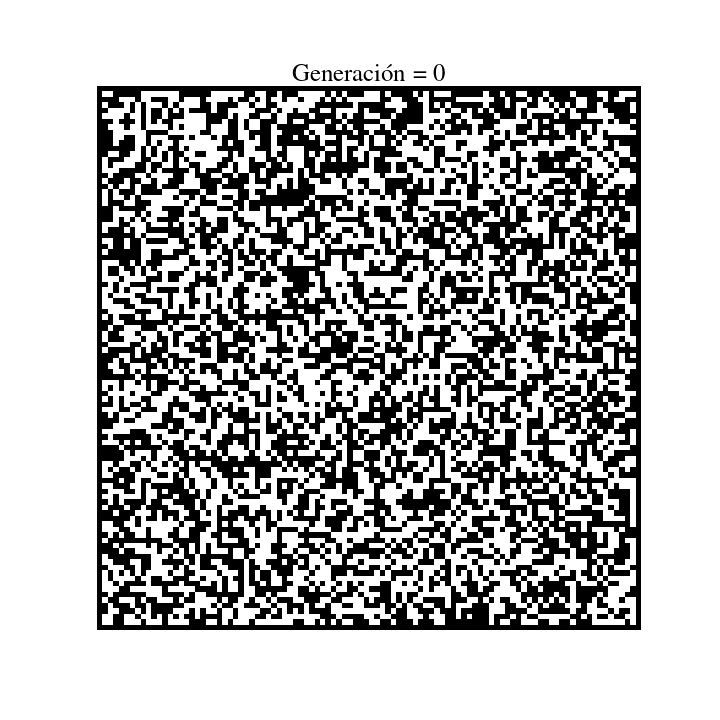
\includegraphics[scale=0.35]{0}
\caption{configuración de dimensión $dim = 100$ con semilla $seed = 1$ en la generación 0.} \label{fig:gen_0}
\end{figure}
\\ 
%
\begin{figure}[h!]
\centering
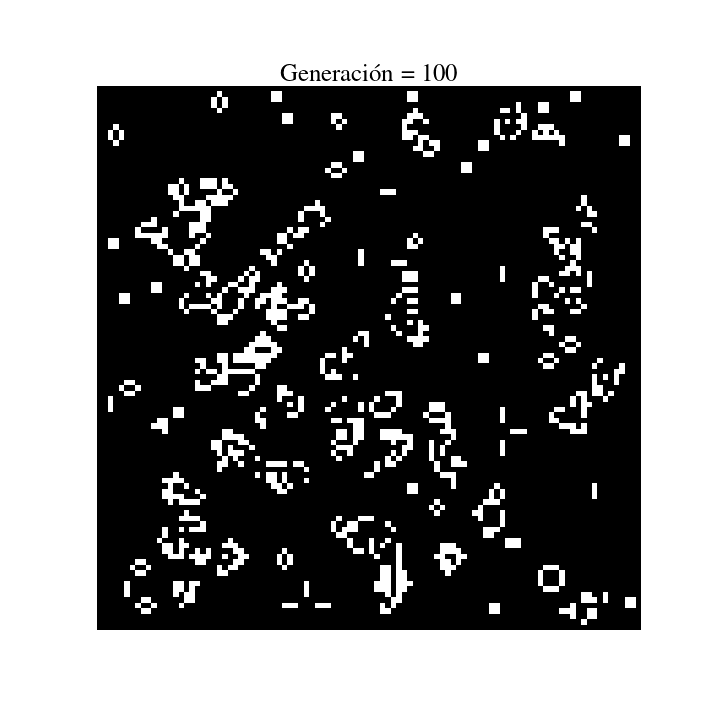
\includegraphics[scale=0.35]{100}
\caption{configuración de dimensión $dim = 100$ con semilla $seed = 1$ en la última generación.} \label{fig:fin}
\end{figure}
\\ 
Con estos resultados se graficó la población viva, el número de muertos y de nacidos en función de la generación, cuyo comportamiento se observa en la figura \ref{fig:graf}
%
\begin{figure}[h!]
\centering
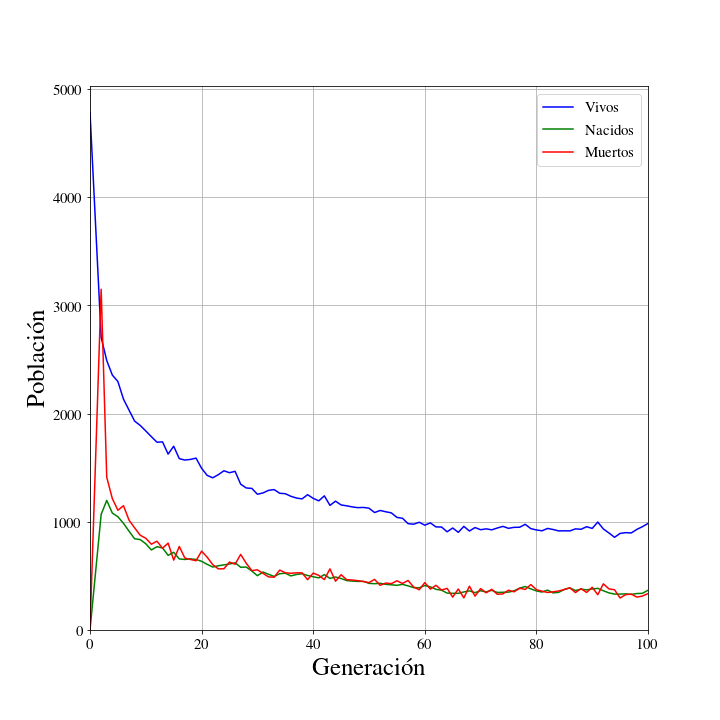
\includegraphics[scale=0.5]{Figures/population}
\caption{gráfico del número de celdas vivas (curva azul), muertas (curva roja) y nacidas (curva verde) en función de la generación.}\label{fig:graf}
\end{figure}
\\
A partir de esta puede observarse un pico en rojo que sobrepasa las 3000 celdas, debido a la gran cantidad de celdas blancas que mueren por sobrepoblación; así como un pico verde más chico sobre las mil celdas. Es interesante observar el comportamiento convergente de los compartimentos: la curva de vivos tiende a mil a partir de la sexagésima generación, mientras que el número de celdas que nacen se equilibran con las que mueren, aportando cada una alrededor de quinientas celdas. Esto indica que esta configuración alcanza un estado cuasiestable, tal vez con algunas regiones oscilatorias y otras estáticas. La evolución de esta configuración inicial está disponible en el gif adjunto.

\end{document}
